\documentclass[DM,lsstdraft,authoryear,toc]{lsstdoc}
% lsstdoc documentation: https://lsst-texmf.lsst.io/lsstdoc.html

% Package imports go here.
\usepackage{graphicx}
\usepackage{url}
\usepackage{latexsym}
\usepackage{color}
\usepackage{enumitem}

% Local commands go here.

% To add a short-form title:
% \title[Short title]{Title}
\title[Alerts Menu]{LSST Alerts: Science-Driven Options for Packets and their Distribution}

% Optional subtitle
% \setDocSubtitle{A subtitle}

\author{%
M.~L.~Graham, T. Pritchard, and the Data Management System Science Team
}

\setDocRef{DMTN-TBD}
\date{\today}
% Optional: name of the document's curator
% \setDocCurator{The Curator of this Document}
\setDocUpstreamLocation{\url{https://github.com/lsst-dm/dmtn-xxx}}

\setDocAbstract{%
\textcolor{red}{\bf EXTREME DRAFT STATE. DO NOT CITE. DO NOT READ. LOOK AWAY.}\\
A review and discussion of the variety of options for alert packets and their distribution, such as latency timescale, packet contents, pre-stream filtering, and so forth.
}

% Change history defined here.
% Order: oldest first.
% Fields: VERSION, DATE, DESCRIPTION, OWNER NAME.
% See LPM-51 for version number policy.
\setDocChangeRecord{%
  \addtohist{0}{2019-11-14}{Conception.}{Melissa Graham}
}

\begin{document}

% Create the title page.
% Table of contents is added automatically with the "toc" class option.
\maketitle

% % % % % % % % % % % % % % % % % % % % % % % % % %
\section{Introduction} \label{sec:intro}

The LSST Science Requirements Document \citedsp{LPM-17} specifies that information about the detections of transient, variable, and moving objects be released promptly as a data stream.

The purpose of this document is to consider the science motivation for, and impact of, the various options for alert packet contents and distribution timescales. 

The contents and delivery of alert packets play a major role in the scientific impact potential of LSST, in part because they are the only LSST data product that is both world public --- they are exempt from any proprietary period --- and publicly accessible -- they are distributed to community brokers, and not solely available via the LSST Science Platform (LSP). In comparison, although the contents of the Prompt products database (PPDB) from which alerts are generated are also world public, access to the PPDB is restricted to individuals with data rights \citedsp{LDO-013} who have authenticated accounts in the LSP.

It is a requirement\reqparam{numStreams}\dmreq{0391} that the DMS be capable of supporting the transmission of at least 5 full alert streams within 60 seconds of image readout. This is based in part on estimates of the alert stream data rate and the bandwidth allocated to alert distribution in the LSST data facility. The size and latency of alerts could therefore affect the ultimate number of supported community alert brokers. 

This draft contains content pertaining to the following open tickets in the DM-SST epic "Studies Around Alerts" (assignees):
\begin{itemize}
\item DM-19484, Estimate distribution of alert packet size based on scientific considerations (Bellm)
\item DM-15654, Define policy for handling fields with $>$10K alerts (Bellm)
\item DM-20296, Investigate the possibility of providing filtered streams (Graham)
\item DM-20298, Revise the contents of the alert packets (Graham)
\item DM-20299, Scientific use-cases requiring $<$5 minute access (Graham)
\item DM-20300, Investigate options for expanding access to the alert stream (Bellm)
\end{itemize}

% \lsrreq \ossreq \dmreq \reqparam 



\clearpage
% % % % % % % % % % % % % % % % % % % % % % % % % %
\section{Alert Packet Contents} \label{sec:packets}

The section explores the science impacts of various options for alert packet contents, such as the $\sim$12 month history of {\tt DIASource} records, the image stamps, and the static-sky {\tt Object} catalog associations.
Reducing the size of an alert packet might be scientifically beneficial if it enables the stream to be transmitted to more community brokers, thereby leading to more science being done with alerts.
It might also be beneficial if it enables brokers to spend less time developing software or spend less of their computational resources to remove parts of the alert packet they do not need prior to processing, and spend more on developing and running algorithms for various alerts-related science goals.
\S~\ref{ssec:packets_remove} and \ref{ssec:packets_compress} consider reducing the size of alert packets by relocating some data or compressing the packets, respectively. 
A small increase to the size of the alert packet is not necessarily going to be scientifically detrimental if the information added enables science, and \S~\ref{ssec:packets_add} considers some small additions regarding the association of {\tt DIASources} with the data release {\tt Object} catalog.

\subsection{Removing Histories and/or Stamps}\label{ssec:packets_remove}

The size of a fully-loaded individual alert packet is estimated to be $\lesssim$82~KB, based on simulations of the planned content of the alerts as described in Section 3.5 of \citeds{LSE-163} (see also \citeds{DMTN-102}). The two largest components of the alert packet which could be considered ``optional'' are the history and the postage stamps. The history is the past $\sim$12 months of {\tt DIASource} records, previously released as alerts. The postage stamps are, at minimum, 30$\times$30 pixels and contain flux, variance, and mask extensions for both the template and difference image, plus a header of metadata \citedsp{LSE-163}. The history accounts for $\sim$27KB of the alert packet ($\sim$33\%) and the stamps contribute $\gtrsim$18~KB ($\sim$20\%). 

Brokers that save all alerts, build their own a database of alerts contents, or have an automated interface with the LSST Prompt products database or Alerts database might not need the historical records to be included in the alert packets. Brokers which do not use the image stamps -- or would need them for only a subset of the alerts and could feasibly query a stamps database -- might not need them included in the alerts packets. Individual broker teams may indicate which information they require (or would like removed from the packets in their stream) during the broker proposal process \citedsp{LDM-612,LDM-682,LDM-723}. During the first stages of the proposal process, and at the LSST Community Brokers Workshop\footnote{\url{ls.st/cbw}} in June 2019, there was some indication that at least a few brokers were interested in alerts without historical records and/or postage historical records.

\subsubsection{{\tt DIASource} Record History}\label{sssec:packets_remove_hist}

Including the {\tt DIASource} record history in every alert allows for the \emph{instant assessment} --- without the need to cross-match or query catalogs --- of changes in the objects's location, size, shape, or brightness, provides context for the latest detection (i.e., anomalous or typical), and enables a robust assessment of the likely physical nature of the object (e.g., light curve fits indicating supernova type become more reliable with more observations). 

To remove the {\tt DIASource} record history from an alert would slightly inhibit the scientific assessment of transient/variable objects for brokers that build their own database of alert contents, due to the time required to cross-match with the database. Removing the {\tt DIASource} record history would completely inhibit this kind of analysis for brokers that do not have such storage or processing capabilities. There is also the issue that the association of {\tt DIASources} into {\tt DIAObjects} may change over time, for some objects. For example, rare cases such as multiply-imaged strongly-lensed supernovae, or two unassociated transients/variables that are superimposed along the line of sight, might be blended/separated in poor/good seeing. In such cases, the set of all associated {\tt DIASources} might be improved between one alert and the next. 

{\bf Summary --} The {\tt DIASource} record histories should not be removed from all alert packets, but could be optionally removed at the request of a broker. However, if the record histories are removed, a list of all {\tt DIASource} identifiers (the {\tt diaSourceId}, as in Section 3.3.1 of \citeds{LSE-163}) which are currently associated with the {\tt DIAObject} to which the alert-spawning {\tt DIASource} is associated should be provided (note that this list is \emph{not} part of the {\tt DIAObject} record).


\subsubsection{Forced Photometry History}\label{sssec:packets_remove_fp}

When forced photometry ({\tt DIAForcedSource} record history) is included in an alert packet, it is ``historical" in the sense that it is based on past images and not the image which spawned the alert. However, it is not always redundant information that was previously released in an alert, like the {\tt DIASource} record history. There are two main cases where forced photometry is performed, as described in \citeds{LSE-163}. (1) For all new {\tt DIAObjects}, forced ``pre-covery'' photometry is done in the past 30 days of difference images within 24 hours, stored in the {\tt DIAForcedSource} catalog, and included in all future alert packets associated with that {\tt DIAObject}. (2) For all {\tt DIAObjects} that are not detected\footnote{The detection threshold is a signal-to-noise ratio $\geq$ 5.} in a given difference image, but had a detection in the past $\sim$12 months, forced photometry is done on that difference image. The result is stored in the {\tt DIAForcedSource} catalog, and included in all future alert packets associated with that {\tt DIAObject}. The forced photometry is scientifically valuable because, for example, pre-covery forced photometry provides context for the first detection of a transient/variable, and low-SNR detections can help with photometric classification and prioritization for follow-up observations. 

If a given {\tt DIAObject} is never again detected in a difference image, then the {\tt DIAForceSource} records are never included in an alert packet, but are available to individuals or brokers with access to the PPDB via the LSST Science Platform. If a given {\tt DIAObject} is repeatedly detected in new difference images, then the same {\tt DIAForcedSource} records will be redundantly included in all future alerts (after the first one containing the pre-covery or non-detection forced photometry). For the ``historical" {\tt DIAForcedSource} records, alert content redundancy could be avoided by only including previously undistributed {\tt DIAForcedSource} data in an alert packet. To do this, the Prompt pipeline would have to either compare with the contents of the most recent alert and remove redundant data from the new alert, or flag the {\tt DIAForcedSource} data as ``released" and only add ``unreleased" forced photometry to a alert packet. Both of these options would add processing times to the alert generation pipeline, which is undesirable.

{\bf Summary --} If the decision is made to remove the historical {\tt DIASource} records from alert packets, the {\tt DIAForcedSource} records of forced photometry should always be added to all alerts. This will cause some redundancy in alert contents, but if not included there would be no public access to this scientifically valuable information.


\subsubsection{Postage Stamps}\label{sssec:packets_remove_stamps}

Including the postage stamps in the alert packet allows for the instant assessment of the {\tt DIASource} in the difference and template images, which has a variety of scientific applications. For example, although real/bogus classification of the difference-image sources will be done prior to alert generation, some brokers may still wish to run additional algorithms on the images -- especially in the case of first detections. Brokers might also employ algorithms to classify transients and variables based on the images instead of the photometry (e.g., \citealt{2019PASP..131j8006C}). From the postage stamp images, scientifically useful information can be derived about the trails left by moving objects, or from the 2-dimensional luminosity distribution of spatially evolving objects such as comets, which might not be entirely captured by the {\tt DIASource} elements (see Table 1 in \citeds{LSE-163}). The images also provide context for the {\tt DIASource}, such as host-galaxy morphology or field crowdedness, that can assist with follow-up observations.

If postage stamps were not created during alert production, the only option would be for users to wait until the images are made available (within 24 hours) in the LSP, which would significantly inhibit alerts-based science goals. However, postage stamps are unlikely to be needed for most {\tt DIASources}, the majority of which --- 95\%, according to the breakdown in \citeds{DMTN-102} --- will be stars or asteroids: point sources for which context is not a significant part of their immediate evaluation. An efficient compromise might be for the Prompt pipeline to create the postage stamps during alert generation, and then store them in a publicly accessible database (i.e., outside the LSP) where they can be obtained (via {\tt diaSourceId}) with a latency similar to the alert distribution timescale by anyone, from anywhere, at anytime. 

The expected maximum download rate from this stamp database is estimated by assuming that all 5 community brokers download $\sim$500 stamp sets per visit: $\sim$2500 stamp sets every $\sim$35 seconds. At 18~KB per stamp set, that's a data rate of 10.5 Mbps (for comparison, that's $\sim$5\% of one full alert stream).

{\bf Summary --} The postage stamps could be removed from all alert packets, but they should still be created during Prompt processing and stored in a publicly accessible database where they can be obtained with a latency similar to the alert distribution timescale.


\subsubsection{Pros and Cons of Multiple Alert Formats}\label{sssec:packets_remove_procon}

The above options could either apply to all alert packets, or brokers could choose from the menu and subscribe to a stream with the options they want.
The latter means that LSST distributes multiple types of alert packet formats, and there are benefits and drawbacks to this ``menu" approach.
The LSST currently expects to deliver alert streams to five brokers, and there are four alert packet formats on the table: (i) with histories and stamps, (ii) with histories but without stamps, (iii) without histories but with stamps, and (iv) without histories or stamps. 

From a science perspective, the benefits to allowing brokers to customize their alert packet is that it potentially enables unique science to be done by brokers (e.g., custom stamp-analysis algorithms), and could enable LSST to support $>$5 brokers which might lead to more alerts-related science in general.
One drawback might be that in times of heavy load, full-sized packet streams might be more likely to be delayed, which would be unfair to brokers requiring full-size packets, and could disproportionately affect some science goals more than others.
The fact that not all alert packets are identical might cause some additional bookkeeping considerations for downstream brokers who ingest from multiple community brokers, but should not be detrimental to their science goals.

The technical considerations of how many different alert packet formats it is feasible to create and transmit within the required latency time is left for data management.


\subsection{Additional {\tt Object} Association Information}\label{ssec:packets_add}

The contents of the alert packet as defined in \citeds{LSE-163} includes the following with respect to associations with {\tt Object} catalog from the most recent data release:
\begin{itemize}
\item {\tt nearbyObj} ({\tt unit64[6]}), the {\it "closest {\tt Objects} (3 stars and 3 galaxies) in Data Release database"}
\item {\tt nearbyObjDist} ({\tt float[6]}), the {\it "distances to {\tt nearbyObj}"} in arcseconds
\item {\tt nearbyObjLnP} ({\tt float[6]}), the {\it "natural log of the probability that the observed {\tt DIAObject} is the same as the nearby {\tt Object}"}
\end{itemize}
For the latter, there is a footnote that says {\it "This quantity will be computed by marginalizing over the product of position and proper motion error ellipses of the {\tt Object} and {\tt DIAObject}, assuming an appropriate prior"}.

The current definitions of {\tt nearbyObj}, {\tt nearbyObjDist}, and {\tt nearbyObjLnP} are not as useful as they could be for transients in host galaxies. 
For extragalactic transients, the three nearest galaxies are not always the three most likely host galaxies, and the distance in arcseconds matters less than a separation distance that accounts for the galaxy's luminosity profile.
Furthermore, the definition of {\tt nearbyObjLnP} is only appropriate for static variable point sources (stars): for transients in host galaxies, the observed {\tt DIAObject} will never be ``the same as the nearby {\tt Object}".

Statistically, the most likely host for a given transient is the galaxy which contributes the most optical flux at the transient's location.
This is usually estimated by calculating an offset distance from the nearby galaxies to the transient that is expressed in terms of the galaxy's spatial luminosity profile, and assuming the galaxy with the lowest offset distance is the host.
The following are several options for estimating which nearby galaxy is the most likely host of an extragalactic transient.

{\bf Effective Radius --} Calculate a separation distance that is the radial distance from the core of the galaxy to the location of the transient, divided by the effective radius of the galaxy (i.e., {\tt kronRad90} in the {\tt Objects} table; \citeds{LSE-163}).
The nearby galaxy with the lowest separation distance is the most likely host. This will account for the relative sizes of the potential host galaxies, but not their position angles. 

{\bf Second Moment --} Calculate a separation distance, as in \citet{2006ApJ...648..868S}, based on the two-dimensional luminosity profile of the galaxy.
Where $x_{\rm trans},y_{\rm trans}$ is the location of the transient, and $x_{\rm gal},y_{\rm gal}$ is the center of the galaxy (the first moment; {\tt radec} in the {\tt Object} table), the separation distance is $R^2 = C_{xx} x_r^2 + C_{yy} y_r^2 + C_{xy} x_r y_r$, where $x_r = x_{\rm SN} - x_{\rm gal}$ and $y_r = y_{\rm SN} - y_{\rm gal}$.
The ellipse parameters $C_{xx}$, $C_{yy}$, and $C_{xy}$ can be calculated directly from the second moments of the galaxy luminosity profile ({\tt Ixx}, {\tt Iyy}, and {\tt Ixy} in the {\tt Object} table), e.g., as described in Section 10 of E. Bertin's Source Extractor manual\footnote{Version 2.3: \url{https://www.astromatic.net/pubsvn/software/sextractor/trunk/doc/sextractor.pdf}}.
The nearby galaxy with the lowest separation distance is the most likely host.
This option accounts for both the relative sizes and position angles of the potential host galaxies, and requires only a little more processing. 

{\bf 2D Algorithms --} There are also other, more complicated methods for identifying the most likely host for a given transient.
For example, the nearby galaxy with the smallest fraction of light interior to an isophot through the transient's location, where the isophot shape is given more degrees of freedom and not constrained to concentric ellipticals as in the second moment method above.
Another example is to use an algorithm that provides deblended footprints for nearby extended objects, and can estimate the fraction of light in given pixel that should be attributed to each (e.g., the SCARLET deblender, \cite{2018A&C....24..129M}).
The most likely host galaxy would be the one which contributes the most flux at the pixel location of a transient.

Generally, nearby galaxies with separation distances $>$3, or $>$99\% of the luminosity profile, are not assigned as hosts and the transient is considered "hostless".
While this cutoff has been appropriate for past samples of $\sim$hundreds of transients, it will not be appropriate for the LSST sample size, and no such cut should be applied when evaluating potential host galaxies for {\tt DIAObjects}. 

All of the above host galaxy identification methods can also make use of priors if the transient type is known; for example, the established correlation between core-collapse supernovae and star formation.
However, such a robust level of host associations are beyond scope for the Prompt pipeline, and the main goal is to provide brokers with sufficient information to assess the potential host association, and decide whether it is useful to the classification and/or prioritization of alerts for follow-up. 

{\bf Summary --} For the ten nearest {\tt Object} catalog galaxies, a separation distance should be calculated with respect to the transient location, preferably using the second moments of each galaxy's luminosity profile. Two new {\tt DIAObject} catalog elements should be added: {\tt nearbyPotHost}, containing the {\tt objectId} for the three galaxies with the lowest separation distances, and {\tt nearbyPotHostSepDist}, containing the separation distances. An analog for the existing element {\tt nearbyObjLnP}, representing the probability, is not necessary. This would add {\tt unit64[3]} and {\tt float[3]} to the {\tt DIAObject} catalog and to each alert, but this both tiny and worthwhile.


\subsection{Compressing the Alert Packets}\label{ssec:packets_compress}

The application of gzip compression could further reduce the size of a full alert to $\sim$65~KB (80\%; JIRA ticket DM-16280).
Naively, this seems like it would allow 1 more full stream to be transmitted to a broker, and thereby enable more science.
However, the time and computational resources required to compress the alert packets needs to be considered.
For example, gzip compression at 50 MB/s to compress $\sim$10000 alerts would take $\sim$10000 $\times$0.08 MB per alert $/$50 MB/s, or $\sim$16 seconds.
This is significant, considering the alert distribution latency requirement\reqparam{OTT1}\lsrreq{0101}\ossreq{0127}\dmreq{0004} is 60 seconds. 
Furthermore, compressing the alert packets forces brokers to then decompress the alerts on arrival, which would incur further delay.
Science goals requiring very low-latency alerts distribution might be negatively impacted by compression -- see \S~\ref{sec:latency} for a deeper discussion of the science drivers for low-latency alerts.

{\bf Summary --} Since packet compression could induce an additional latency, perhaps it should only be done if, e.g., an algorithm could provide a compression rate of $\lesssim$10 MB/s (requiring only a few seconds to compress a visit's worth of alerts), or if the alert distribution latency requirement is relaxed from 1 minute (see \S~\ref{sec:latency}).
Otherwise, compression would have no impact on alerts-related science goals and so this should be primarily a technically-driven decision.




\clearpage
% % % % % % % % % % % % % % % % % % % % % % % % % %
\section{Alert Distribution Latency} \label{sec:latency}

It is a requirement that the DMS be capable of supporting the distribution of at least 98\%\reqparam{OTT1}\reqparam{OTR1}\lsrreq{0101}\lsrreq{0025}\ossreq{0127}\dmreq{0004} of alerts for each visit within 60 seconds of the end of image readout.

If it is possible to relax this requirement to, e.g., 5 minutes -- \emph{without risk to the science goals} -- then it might be possible to support more community brokers and/or repurpose the human and computational resources that would otherwise be dedicated to delivering 1 minute alert distribution. This section attempts to gather the science goals which might potentially require 1 minute alert distribution and could not be satisfied with a longer latency.

{\bf Generally, science goals that require alerts on timescales shorter than $\sim$5 minutes have that need because they also require follow-up on timescales shorter than $\sim$15--30 minutes.} Most observing strategies for the WFD main survey do not revisit fields on timescales shorter than $\sim$15 minutes (strategies that do pair visits aim for closer to $\sim$22 minute gaps). Thus, any science goals driving the need for alerts on timescales shorter than $\sim$5 minutes \emph{must also be able to confidently identify their targets with single-epoch single-filter LSST photometry}, or be using additional information (such as host galaxy characteristics, or coincidence with another survey's data).

{\bf Target of Opportunity --} It is important to note that for rapid ToO observations with LSST (if they occur), there might not be time to pre-cache slow database queries (e.g., loading slices of the PPDB catalogs) when upcoming pointings are not known in advance, as would happen during regular survey observations. This might mean that a 1 minute alert distribution timescale for alerts from ToO imaging surveys cannot be guaranteed, and this should be kept in mind when reading through the science cases for short alert latencies in this section. \textcolor{red}{$\leftarrow$ This statement was modified from something ECB mentioned on Slack, double check it's accurate}.

\subsection{TVS Survey Results Regarding Alerts Timescales}\label{ssec:latency_tvs}

The Transients and Variable Stars (TVS) science collaboration surveyed the science needs of their members with respect to alert latency, and the results are shown in Table \ref{tab:tvs}\footnote{Results courtesy of TVS co-chair Rachel Street.}. The survey asked respondents to choose the maximum tolerable and ideal average delay between the alerts being produced by the LSST data reduction pipeline and the alert information becoming available through the broker service. This is not exactly the same as the alert distribution timescale {\tt OTT1}, but these responses will inform the need for $<$1 minute alert distribution.  Respondents were asked to provide a short summary of their science goals for alerts if they reported needed access within 15 minutes. Note that the pool of respondents is probably not representative of the wider collaboration, and is likely biased towards individuals with science interests that do require faster access to alerts. 

Only 20\% (10\%) of respondents report that $<$10 minutes ($\leq$1 minute) is an ideal average delay, and whereas 70\% report that $>$30 minutes would be a sufficient average latency. The three science drivers associated with $<$5 minute alert access are the electromagnetic counterparts to gravitational wave events (EM-GW; kilonovae), young supernovae (early short-lived light curve features such as shock breakouts), and gamma-ray bursts (GRB). It is at first confusing that EM-GW was provided as the science driver for such a wide range of alert access timescales, but this is discussed further in \S~\ref{ssec:latency_emgw}, along with several other science cases that rely on rapid access to LSST alerts.

\begin{table}[h]%[htdp]
\caption{Table of results from a TVS survey which asked "how fast do you really need alerts?". The total number of respondents was 20. The science driver acronyms are: EM-GW (electromagnetic counterparts to gravitational wave events), YSNe (young supernovae, including e.g., shock breakouts), GRBs (gamma-ray bursts). \label{tab:tvs}}
\begin{center}
\begin{tabular}{|l|cl|cl|}
\hline
             & Maximum & Science & Ideal       & Science \\
Latency & Tolerable  & Driver(s) &  Average & Driver(s) \\
\hline
1 min or less & 1 & EM-GW, GRB  & 2 & EM-GW, YSNe, GRB \\
1-5 min         & 0 &                          & 1 &                                   \\
5-10 min       & 1 & EM-GW, YSNe & 1 & YSNe \\
10-30 min     & 2 & YSNe               & 2 & EM-GW, GRBs \\
30-60 min     & 2 &                          & 7 & EM-GW  \\
1-6 hours     & 4 & EM-GW, GRBs & 1 &  \\
6-12 hours   & 2 &                          & 1 &  \\
12-24 hours & 3 & EM-GW            & 1 & EM-GW \\
1-3 days      & 1 &                           & 0 &  \\
>3 days       & 4 &                           & 4 &  \\
\hline
\end{tabular}
\end{center}
\label{default}
\end{table}%


\subsection{EM Counterparts to GW Events}\label{ssec:latency_emgw}
% From Slack conversation, Federica Bianco, Om Sharan Salafia, Eric Bellm

During LSST Operations, target-of-opportunity imaging follow-up sequences might be executed in the error ellipse of a gravitational wave (GW) detection to search for the electromagnetic (EM) optical counterpart. Such a search yielded a fast-evolving "kilonova" which decayed from 22 to 28th magnitude in the $g$-band in just 6 days \citep[faster in the bluer and slower in the redder filters][]{2017Sci...358.1559K}. Although the kilonova light curves last only a few days, since there is so far only one event, GW170817, a day or two delay between the GW event and the optical detection still yields very scientifically valuable data -- for now. During LSST Operations there will already exist a sizable collection of longer-latency follow-up, and it is likely that science will be moving in the direction of pushing to ever earlier detections. However, since KNe produce days-long optical afterglows, a 5 minute LSST alerts would likely suffice.

There are two theoretical predictions for prompt optical emission that would require very rapid access to alerts. One of them is a potential faint, $<$1 hour, UV/optical transient that occurs at the time of jet-break out for a short gamma-ray burst associated with a binary neutron star merger (\S~\ref{ssec:latency_grb}). Another that predicts emission of a similar color, luminosity, and timescale is the spin-down energy of a long-lived ($10^2$--$10^4$ s) neutron star formed from a binary neutron star merger before its eventual collapse to a black hole \citep{2016ApJ...819...15S}. As described in \S~\ref{ssec:latency_grb}, very few events could be detected by serendipitous coincidence by the LSST WFD main survey, and targeted follow-up of well-localized GW events with more appropriate facilities (such as space-based UV/optical imagers) is much more likely to yield detections of this very short lived emission.

There are two additional issues related to ToO for EMGW events which might make 1 minute alerts necessary or impossible. First, as described above, for a ToO imaging survey with LSST there might not be time to pre-load catalogs for the targeted fields. The second is that, at least for run O3, the GW event detection system itself issues preliminary alerts within 1--10 minutes, and these preliminary alerts are often retracted and do not always have the sky localization. Even now, many imaging follow-up surveys wait for the initial alert (or retraction) to be sent after a round of human vetting of the GW event signal, and this can take several hours. With such latencies, the 1 {\it vs.} 5 minute LSST alert timescales becomes inconsequential. 



\subsection{Gamma-Ray Bursts}\label{ssec:latency_grb}

For short gamma-ray bursts (sGRBs) which are thought to be the mergers of two neutron stars, or a neutron star and a black hole, as the jet propagates through the ejecta material a hot cocoon is formed. When cocoon and jet break out, along with sGRB can can be observed as a blue transient with an absolute peak brightness of -12 to -15 magnitudes that lasts for $10^3$--$10^4$ seconds (e.g., \citealt{2018MNRAS.473..576G}). For an LSST detection limit of $r\sim24$ mag, a detection limit of $r\lesssim-12$ ($r\lesssim-15$) mag corresponds to distances of $\lesssim160$ ($\lesssim630$) Mpc, or redshifts $z\lesssim0.035$ ($z\lesssim0.14$). Observing the diversity of cocoon emission will require multi-band follow-up within $10^3$ seconds, or $15$ minutes, and in this particular case a 5 minute alert distribution latency is too long to include the shorter events (or the fainter events for which only the peak would be visible).

% z=0.035 is V=0.014 Gpc3
% z=0.14 is V=0.836 Gpc3
% (0.836/0.014) * 4/yr = 240/yr

The rate of short GRBs in the local volume ($<$200 Mpc) is estimated to be quite low, $<$4 $\rm yr^{-1}$ \citep{2019arXiv190800100M}. Scaling this up to the co-moving volume within 630 Mpc is $\sim$240 $\rm yr^{-1}$, all-sky. In the baseline main survey, about a sixth of the sky can be observed in a given night, which is $\lesssim$0.1 event in the WFD main survey area per night. With $\sim$1000 visits per night, and $\sim$10 visits every 5 minutes, there's a $10^{-3}$ chance that the location of a sGRB will be serendipitously observed within 5 minutes of the event on a given night. So this could happen once every 3 years, or $\sim$3 times over the 10-year LSST main survey.

For this particular science case, LSST seems to be the wrong tool for the job. As described by \citet{2018MNRAS.473..576G}, a rapid search at the location of sGRBs with a UV satellite such as ULTRASAT would be ideal.

%Triggering criteria might be:
%new {\it u}- or {\it g}-band source with recent limits associated with a $<$200 Mpc galaxy (how many expected per night?)
%and then very high priority if it's serendipidously associated with a GRB detection in the last 5 minutes


\subsection{Young Supernovae}\label{ssec:latency_ysne}


\subsection{Fast Radio Bursts}\label{ssec:latency_frb}

One of the strongest -- but also most mysterious -- transients that might significantly benefit from the $60$ second alert timescale are fast radio bursts (FRBs): a millisecond long pulse of coherent emission in the GHz range.
The emission is dispersed by the inter-galactic medium (IGM), such that the pulse's observed arrival time is frequency dependent.
Observed FRB dispersion measures of $\rm{DM}\approx100$ to $1000$ $\rm pc\ cm^{-3}$ indicate that their origins are at cosmological distances, with redshifts $z\approx0.1$ to $1$ \citep{2018Natur.562..386S}. 

If an optical counterpart is generated by this coherent emission, the time delay between the optical detection and the radio detection is on the timescale of minutes for frequencies $\nu < 500\ {\rm MHz}$, as shown in Figure \ref{fig:sci_frb}.
This leaves open the possibility for triggering radio follow-up of optical counterpart candidates -- if they exist and are detectable -- and triggering additional follow-up for a serendipitous co-detection of FRB and optical transient.
A millisecond-long event in the optical would have to be quite bright to be detected by LSST, but studies show that LSST detections are feasible \citep{2016ApJ...824L..18L}.
\cite{2019ApJ...878...89Y} demonstrate that two theoretical sources for coherent optical emission from FRBs would not be detectable by LSST, but that inverse Compton scattering processes could lead to optical detections with LSST (e.g., from pulsars or masers).
If FRBs are associated with superluminous supernovae (SLSNe) and young magnetars, then potentially an LSST alert regarding a change in behavior of known SLSNe could be used to trigger radio follow-up.
However, this case is unlikely to be as sensitive to the LSST alert distribution timescale as the optical emission would be released over a longer time window \citep{2019arXiv191002036L}.

Searches for FRB counterparts in optical images that were serendipitously obtained coincidentally with an FRB detection have only just recently become possible thanks to current wide-field imaging surveys.
No transient optical counterparts have yet been detected \citep{2019ApJ...881...30T}, but individual host galaxies for FRB events have been identified \citep{2016Natur.530..453K}.
Since the rate of FRBs is estimated to be quite high, thousands per day \citep{2016MNRAS.460L..30C}, even after radio detection efficiency is factored in there should be many within the observed LSST volume.

\textcolor{red}{\bf Need an estimate of the number of FRB locations serendipitously observed by LSST within a few minutes window.}

\begin{figure}[h]
\begin{center}
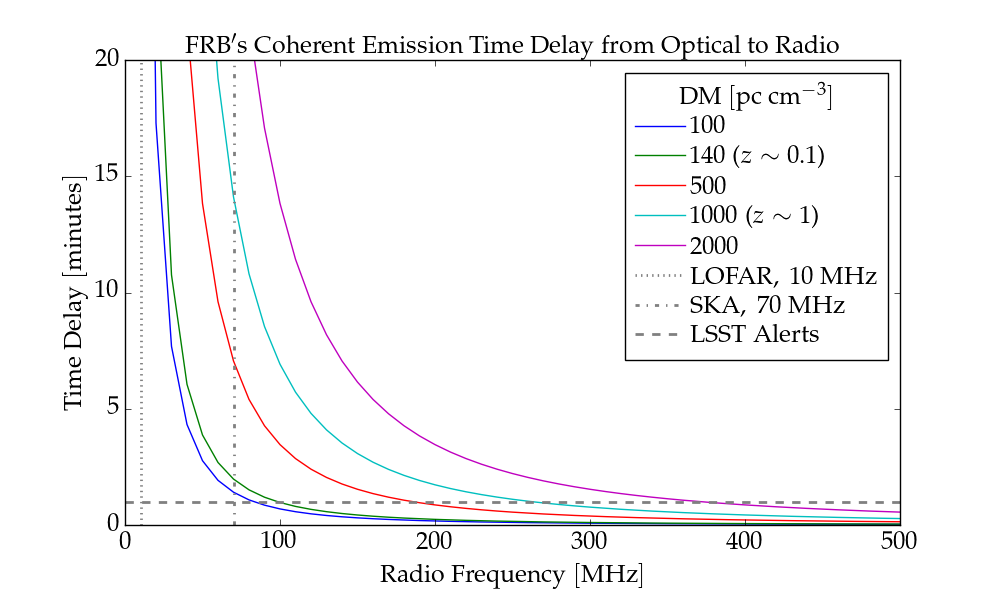
\includegraphics[width=12cm]{figures/frb_optical_delays.png}
\caption{The delay time (for coherent emission) between the arrival of the optical and radio photons due to cosmological dispersion, as a function of the frequency of the radio detector. The {\it lowest} frequency bands of the Square Kilometer Array (SKA) and the Low-Frequency Array (LOFAR) are marked with vertical dotted and dash-dotted lines, and the 1 minute timescale for LSST alert distribution with a horizontal dashed line. The delay time is $\Delta t = k_{\rm DM}\,DM\,(\nu_{\rm low}^{-2} - \nu_{\rm high}^{-2})$, where $k_{DM}=4.149$ $\rm GHz^2\ pc^{-1}\ cm^3\ ms$, ${\rm DM}$ is the dispersion measure in $\rm pc\ cm^{-3}$, $\nu$ is the low and high frequency bands of the observation, and $\Delta t$ is in $\rm ms$. We have used the range of FRB dispersion measures as observed by \cite{2018Natur.562..386S}. \label{fig:sci_frb}}
\end{center}
\end{figure}

\subsection{Solar System Objects}\label{ssec:latency_sso}

\textcolor{red}{MLG: in Lynne's talk on the SSSC needs for alerts brokers at the CBW in June 2019, slide 4 says that a needed broker capability was "API or other 'push' notification (e.g., trailed detections) [minutes may count]". Follow-up on the SS use case for alerts on very short timescales.}


\subsection{Summary}\label{ssec:latency_summary}




\clearpage
% % % % % % % % % % % % % % % % % % % % % % % % % %
\section{Pre-Filtered Alert Streams} \label{sec:prefilter}

Pre-filtered streams might mean the alerts can be distributed to more brokers than numStreams. What kind of pre-filters might suit the brokers?

 - magnitude or signal-to-noise ratio (affects completeness/purity)
 - region of sky (like one of the LOI for a particular region)
 - static-sky object association
 
 Image free streams of alert packets.
 Sources only associated with past alerts.

Provide estimates for how much the alert stream volume would be reduced.



\clearpage
% % % % % % % % % % % % % % % % % % % % % % % % % %
\section{Graceful Degradation} \label{sec:graceful}

Along with the requirement of a 60 second alert distribution timescale (\S~\ref{sec:latency}, the DMS should support the distribution\reqparam{transN}\lsrreq{0101}\reqparam{nAlertVisitAvg}\ossreq{0193}\reqparam{nAlertVisitPeak}\dmreq{0393} of at least 10,000 alerts per standard visit on average during a given night, and at least 40,000 alerts per single standard visit. 

It is also a requirement\reqparam{sciVisitAlertDelay}\reqparam{sciVisitAlertFailure}\ossreq{0112}\dmreq{0392} that no more than 1\% of all standard visits fail to have at least 98\% of its alerts distributed within 60 seconds of image readout, and that no more than 0.1\% of all standard visits fail to distribute alerts.

These requirements apply to standard visits which should have produced $\leq$40,000 alerts. For example, a visit would be considered "delayed" and count towards that 1\% limit if $>$2\% of its alerts were distributed with a latency of $>$60 seconds. The requirement that no more than 0.1\% of all science visits fail to generate and/or distribute alerts is integrated over all stages of data handling, not just alert distribution, and includes failures at any stage of prompt processing.

It is furthermore specified that alert distribution "degrade gracefully" beyond that limit, meaning that visits resulting in an excess of alerts should not cause any DMS downtime \citedsp{LSE-30,LSE-61}.


In crowded fields there might be $>$40,000 difference-image sources.

For alerts that are not distributed within 60 seconds, how should they be handled? 

It is a requirement that all alerts be stored in an archival database and be available for retrieval\ossreq{0185}. The term "available for retrieval" applies to users with data rights and access to the LSST Science Platform. Like all other Prompt data products, the alerts archive will be updated within 24\reqparam{L1PublicT}\lsrreq{0104} hours \citedsp{LSE-29}.

\textcolor{red}{From the community post brokers FAQ $\rightarrow$}The retention period in the alert distribution system is still to be determined, but given the alert stream data rate of ~800 GB/night it is currently reasonable to expect a retention period of ~7 days. Brokers with data rights can retrieve old alert packets from the Alerts Database. However, note that the requirements on user access to the Alert Database are not yet fully developed, and may be limited in terms of how alert packets may be queried (e.g., alert ID), or by the bulk download capabilities (DMTN-102 1).



\clearpage
% % % % % % % % % % % % % % % % % % % % % % % % % %
\section{LSST Alert Filtering Service}\label{sec:lafs}

It is a requirement that the LSST alert filtering service be able to support\reqparam{numBrokerUsers}\dmreq{0343} at least 100 simultaneous users. The LAFS will be capable of returning 20\reqparam{numBrokerAlerts}\dmreq{0343} full-sized alerts per visit per user.

The LSST alerts filtering service is a mechanism by which users --- individuals with LSST data rights and access --- can receive alerts via pre-defined filters that have been optimized for established transient classifications such as supernovae and/or create and apply their own filters to the stream \citedsp{LPM-17,LSE-61}. 

Which options might be appropriate for implementation with the LAFS?
A few of these options might also be available to users of the LSST alert filtering service (\S~\ref{sec:LAFS}).


% Include all the relevant bib files.
% https://lsst-texmf.lsst.io/lsstdoc.html#bibliographies
\bibliography{local,lsst,lsst-dm,refs_ads,refs,books}

\end{document}
